\chapter{研究の目的}\label{chap:purpose}
%@@@1章の節にしましょう。

走行箇所である畦道から外れて走行することを防ぐために画像中から畦道領域を取得
水田への落下を防ぐために畦道領域の取得と路面状況の評価を併用し走行可能な路面を検出すること
\\
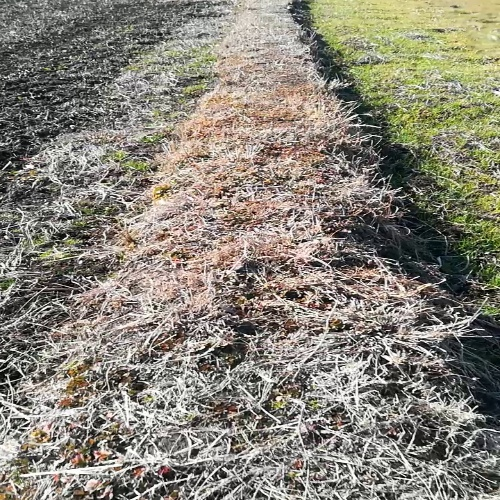
\includegraphics[width=5cm]{figs/fig1.jpg}

%@@@なんで体言止めなの?
%@@@(文になってないけど)文が長すぎて意味不明
%@@@図について全く言及がない(この図は1.1へ。でもこれ、草ぼーぼーじゃないね。)
